\section{Физический вакуум. Эффект Казимира}

%%%%%%%%%%%%%%%%%%%%%%%%%%%%%%%%%%%%%%%%%%%%%%%%
\subsection{Теория поля и квантовая теория поля}
Для упрощения восприятия многих вопросов, упоминаемых в данном тексте, будет полезно иметь некоторое представление об объектах, с которыми придется работать во избежание принципиально ошибочных интерпретаций. 
Стартовать с нуля невозможно, поэтому предполагается, что читатель знаком с классической теоретической физикой и нерелятивистской квантовой механикой. 

В теоретической физике основными инструментами были лагранжиан, который для системы с $n$ степенями свободы зависел от $n$ обобщенных координат и их производных по времени $L = L(q_1, \ldots, q_n, \dot{q}_1, \ldots, \dot{q}_n)$, и интеграл по времени от него -- действие $S = \int L\d t$. 
Из принципа наименьшего действия получались уравнения эволюции системы
\begin{equation}
\frac{\d}{\d t} \left(\frac{\partial L}{\partial \dot{q_i}}\right) - \frac{\partial L}{\partial q_i} = 0 ,
\quad
i = \overline{1,n}
.
\label{eq:q.evolution}
\end{equation}
Классическая теория поля, условно говоря, представляет собой переход к бесконечному числу степеней свободы, когда набор обобщенных координат $q_i$ заменяется на поле $\phi(\vec{x}, t)$, где $\vec{x}$~-- радиус-вектор, а их производные по времени $\dot{q}_i$~-- на частные производные поля по всем переменным. 
Вместо лагранжиана $L$ в этом случае удобно рассматривать его плотность $\L$. 
Тогда действие принимает вид 
$$
S = \int L(\phi, \partial\phi) \d t = \int \L(\phi, \partial\phi) \d^3 \vec{x} \d t = \int \L(\phi, \partial\phi) \d^4x,
$$
где $x$ -- четырехвектор в пространстве-времени. 
Принцип наименьшего действия приводит к уравнению
\begin{equation}
\sum\limits_{\mu=0}^{3}\frac{\partial}{\partial x^\mu} \left(\frac{\partial \L}{\partial \left(\frac{\partial \phi}{\partial x^\mu}\right)}\right) - \frac{\partial \L}{\partial\phi} = 0 ,
\label{eq:phi.evolution}
\end{equation}
очень похожему на~(\ref{eq:q.evolution}), но в явном виде инвариантному относительно преобразований Лоренца.
Как видно из приведенных формул, смысл разделять время и пространство полностью пропадает, теория становится более приспособленной к релятивистскому рассмотрению. 

Теперь, осуществляя переход к квантовой теории, как это было с квантовой механикой, все величины нужно заменить соответствующими операторами. 
Выходит, что лагранжиан сам по себе зависит от операторов, и по ним придется дифференцировать. 
К тому же, уравнения эволюции системы, аналогичные~(\ref{eq:phi.evolution}), содержат теперь только операторы. 
Это, на первый взгляд, порождает довольно сложную интерпретацию любых процедур и результатов, однако на помощь приходят теория возмущений и диаграммы Фейнмана. 
Последовательно примененные операторы $\phi(x_i)\,\phi(x_{i-1})\ldots\phi(x_1)$, усредненные по квантовому состоянию, будут выражать амплитуду вероятности прохождения частицы через точки $x_1, \ldots, x_i$.

Единственным объектом, определяющим свойства полей, а с ними и частиц, является лагранжиан. 
Все характеристики процессов, включая константы взаимодействия и массы частиц, будут определяться его формой. 
Осознавая это, гораздо проще воспринимать изменения этих параметров в различных ситуациях. 


%%%%%%%%%%%%%%%%%%%%%%%%%%%%%%%%
\subsection{Виртуальные частицы}

В квантовой теории поля точное решение существует лишь для небольшого набора модельных гамильтонианов, которые зачастую далеки от нужных для описания эксперимента. 
Однако, относительно простой задачей является рассмотрение ни с чем не взаимодействующего поля. 
Если имеется решение для этого случая и если взаимодействие не слишком велико, полноценный гамильтониан всех необходимых полей с учетом их взаимодействия можно представить в виде суммы гамильтониана невзаимодействующих полей и гамильтониана взаимодействия, который из-за малости можно рассматривать как возмущение. 
Тогда можно решать задачу, применяя теорию возмущений. 

\begin{figure}
\def\svgwidth{.5\linewidth}
\input{figs/VirGamma.pdf_tex}
\caption{Пример виртуальной частицы в диаграмме Фейнмана.}
\label{fig:VirGamma}
\end{figure}

В этом случае квантовая теория поля допускает интерпретацию взаимодействия частиц как обмена виртуальной частицей (или несколькими). 
Виртуальной называется частица, которая и рождается, и умирает в пределах одной диаграммы Фейнмана, например, как $\gamma$-квант на Рис.~\ref{fig:VirGamma}. 

Многие квантовые числа виртуальных частиц могут не совпадать с привычными нам. 
Например, виртуальный $\gamma$-квант может иметь продольную поляризацию, отличный от единицы спин, ненулевой или даже отрицательный квадрат четырехимпульса $p^2$, который для реальных частиц равен квадрату массы. 
Никакие характеристики виртуальных частиц нельзя измерить физическими приборами, об их существовании можно судить лишь по согласию эксперимента и основанных на их участии в реакции расчетах. 
Вероятность возникновения виртуальных частиц зависит от величины константы взаимодействия, из-за которого они возникли, и их импульса. 
Например, амплитуда вероятности может содержать множитель 
$$ \frac{1}{p^2 - m^2}, $$
где $p$ -- четырехимпульс виртуальной частицы, а $m$ -- масса реальной. 


%%%%%%%%%%%%%%%%%%%%%%%%%%%%%%%
\subsection{Содержимое вакуума}

В отличие от классической физики, в квантовой теории допускается случай, когда единственная частица и испускает, и поглощает виртуальный квант поля (однако это не означает, что частица может действовать на саму себя). 
И, что еще важнее, если гамильтониан содержит, например, поле фермионов, поле бозонов и их взаимодействие, то даже в основном состоянии (вакууме) получающейся системы могут возникать виртуальные пары частица-античастица. 
Подобные ситуации обусловлены присутствием квантовых полей даже в вакууме.

\begin{figure}[b]
\includegraphics[width=.5\linewidth]{figs/gamma-to-ee}
\caption{Превращение виртуального фотона в электрон-позитронную пару.}
\label{fig:gamma-to-ee}
\end{figure}

Для начала обсудим немного более простой случай -- взаимодействие двух заряженных частиц.
Для иллюстрации будем считать, что все возможные заряженные частицы -- электроны и позитроны. 
Простейший случай обмена виртуальным фотоном изображен на Рис.~\ref{fig:VirGamma}. 
Такой прямой обмен не приводит ни к каким неожиданным явлениям и поэтому не представляет особого интереса. 
Одно из возможных усложнений -- превращение виртуального фотона ``по пути'' в электрон-позитронную пару, как показано на Рис.~\ref{fig:gamma-to-ee}. 
В этом случае виртуальный фотон часть времени проводит в виде электрон-позитронной пары, что влияет на результирующий эффективный потенциал, который ощущают обе взаимодействующие частицы. 
Учет диаграмм такого типа приводит к, на первый взгляд, неожиданным последствиям -- видимый заряд частиц уменьшается. 

\begin{figure}
\def\svgwidth{.5\linewidth}
\input{figs/VacPol.pdf_tex}
\caption{Поляризация вакуума вокруг заряженной частицы и экранировка ее истинного заряда.}
\label{fig:VacPol}
\end{figure}

Осознать результат можно следующим образом. 
Так как виртуальный фотон может превратиться в электрон-позитронную пару в какой угодно точке, можно считать, что пространство заполнено множеством электрон-позитронных пар, которые в каком-то приближении являются маленькими диполями. 
Поскольку, например, электрон, имеет отрицательный заряд, эти диполи будут ориентированы положительной стороной к нему, пространство вокруг электрона будет иметь поляризацию и станет экранировать настоящий заряд, как показано на Рис.~\ref{fig:VacPol}. 
Это явление известно как поляризация вакуума. 

Возникновение виртуальных частиц в вакууме выглядит примерно так же. 
Рождающиеся частицы либо сами взаимодействуют с чем-то, либо рождают другие. 
Этот процесс называют квантовыми флуктуациями. 
В результате них, когда реальная частица попадает в какую-то область пространства, она не существует одна, а становится окружена множеством виртуальных, которые из-за наличия взаимодействия с реальной перераспределяются, как это делали электрон-позитронные пары, и изменяют видимые характеристики частицы. 
Так происходит, например, с магнитным моментом. 
Спиновый магнитный момент свободного электрона не равен $\mu_B$, то есть спиновый фактор Ланде $g_s$ не равен в точности $2$, в отличие от предсказаний теории Дирака. Влияние на него оказывают виртуальные частицы вакуума и диаграммы, подобные изображенной на Рис.~\ref{fig:g_s}, поскольку они как бы ``размывают'' электрон в пространстве. 
Относительное отличие фактора Ланде электрона от двойки $a_e = \frac{g_s - 2}{2}$ является одним из наиболее точных результатов, подтверждающих квантовую теорию поля. 
Теория и эксперимент согласуются вплоть до 12-го порядка~\cite{electron.g-2.exp, electron.g-2.theory}
\begin{align*}
a_e^\text{теор.} &= 0.001\,159\,652\,181\,643\ (763), \\
a_e^\text{эксп.} &= 0.001\,159\,652\,180\,73\ (28). 
\end{align*}

\begin{figure}
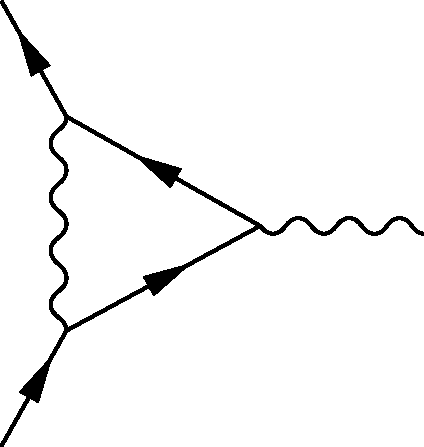
\includegraphics[width=.25\linewidth]{figs/Magnetic-anom-e}
\caption{Простейшая диаграмма, дающая вклад в аномальный магнитный момент фермионов.}
\label{fig:g_s}
\end{figure}

Еще одно экспериментальное подтверждение теории связано со спектром атома водорода. 
Как известно, уровни энергии в этой системе с учетом спина электрона зависят от главного квантового числа $n$ и полного момента электрона $j$, но не от его орбитального момента $l$. 
Это случайное вырождение по $l$ обусловлено не симметрией потенциала, а показателем степенной зависимости его от расстояния между частицами. 
И это вырождение снимается при учете нескольких явлений квантовой электродинамики. 
Впервые зависимость энергии от орбитального момента электрона была экспериментально обнаружена для уровней $2s_{1/2}$, $2p_{1/2}$ Лэмбом и Ризерфордом~\cite{LambShift.exp}, а смещение этих уровней в спектре было названо лэмбовским сдвигом. 
%
Теория объясняет это следующим образом.
Из-за поляризации вакуума потенциал кулоновского взаимодействия точечных частиц имеет близкое к дельта-функции слагаемое при нулевом расстоянии между ними. 
Оно приводит к смещению $S$ уровней, поскольку для них $\psi(\vec{x}=0)\neq0$. 
Однако, учет неточечности протона осложняет ситуацию и уменьшает конечный вклад, в итоге эта часть смещения довольно мала. 
Большее влияние оказывает взаимодействие электрона с квантовыми флуктуациями вакуума. 
Их можно приблизительно считать малыми колебаниями электрона, которые в его собственной системе отсчета (которая с достаточной точностью близка к инерциальной) видны как малые колебания ядра, и поэтому тоже дают вклад только в $S$ уровни электрона. 
Изучение лэмбовского сдвига важно, поскольку он связан в основном с квантовыми флуктуациями, поведение которых представляет большой интерес. 
Для примера их важности достаточно упомянуть излучение частиц черными дырами, предложенное Стивеном Хокингом~\cite{Hawking}.

